\section{The Coding Problem}

The coding problem is the challenge of designing codes that can efficiently and reliably transmit data over noisy channels. To do this, we try to maximize the rate of transfer $R$ which involves increasing $k$ and reducing $n$ while simultaneously increasing the distance $d$ to allow us to correct more errors. \\

\subsection{Example}


Let's give a simple example of us encoding and decoding by talking. We define a Discrete Memoryless Channel (DMC) where the alphabet is the entire dictionary, so every word is a symbol. Then we define our noise function as the following: Every symbol has a probability let's say $p = \frac{1}{4}$ to have an error, meaning that symbol would be replaced by a random other symbol (the distribution does not matter here as this is not formal and is purely for your understanding). For example, if the word 'play' was rolled as an error, it could become 'exfoliating' or 'mouse' or 'summer', etc. \\

Now given this context, Bob wants to tell Alice 'wanna play basketball' over this channel, but Alice could hear 'never play basketball'. How can we correct or detect the error? One way is by using a repetition code. This involves sending multiple copies of each symbol, and the receiving end would choose the symbol that appears most commonly in each group of 3. Now Alice hears: 'wanna never wanna play play play basketball football basketball', she decodes the message and hears 'wanna play basketball'. No more errors! However, notice this adds redundancy to the data we're sending, which makes it far less efficient. If our channel becomes noisier, let's say $p \ge \frac{1}{3}$ then our code will almost never work and we'd need to add more redundancy by sending more copies to ensure transmission is reliable enough.  \\

Most engineers tinkered and tried to create the ideal code by varying the ratio of information bits to redundant bits and testing the reliability, but Shannon was the only one to ask 'What is the thoeretical maximum rate of information I can have whilst still being reliable?'.  \\


\subsection{Exploring Reliability}
The reasoning of why maximizing $R$ increases our rate of transfer is trivial, however, why does increasing the distance improve the reliability of the code? To explore this idea, let us select a random encoding and decoding function, $E$ and $D$ for every message $\mathbf{u}$ of length k. The codeword $E(u)$ is chosen randomly from the set of all codewords with uniform probabilities. The decoding function is maximum likelihood decoding, which is also known as minimum distance decoding outlined in the preliminaries section. Please follow alongside Figure \ref{fig:ball2} for the following section.\\

Suppose we send codeword $E(u)$ and it is received on the other end as $y$. Now draw a Hamming ball with radius $pn$ - the expected number of bit flips after transmission - and center at $E(u)$. Observe Figure \ref{fig:ball2} for a visualization of what we are doing. By Chernoff Bounds, we know that $y$ is almost certainly within our ball. \\

Next, draw another ball around $y$ of the same radius $pn$. The only scenario where our decoding function could fail is when there is another codeword $E(u')$ that is within a ball of radius $pn$ around $y$. \\

As we increase k, we also increase the number of valid codewords. This increase in density reduces the minimum distance. \\

Here we are viewing the same problem of trading off efficiency for reliability from a different perspective.\\


\begin{figure}
    \centering
    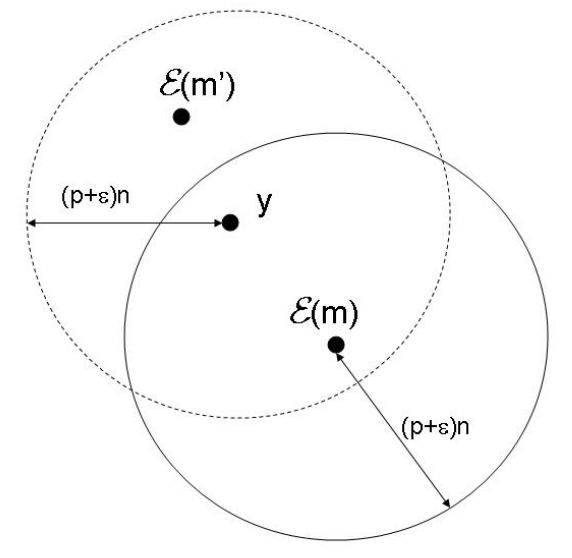
\includegraphics[width=0.5\linewidth]{images/hammingballs.png}
    \caption{Hamming balls with received message $y$ and sent message $E(x)$}
    \label{fig:ball2}
\end{figure}

\textit{Note: you can imagine $y$ drifting away from the original codeword as it's being sent, then once received, it is matched with the closest codeword and decoded, this is the principle of what is happening above.}
